\subsection{Error Detection and Correction}
One of the big challenges of physically realising a quantum 
computer is its subjection to noise in the real world.
Unlike classical computers, the type of error is not limited
to a bitflip, as even single qubit states have a theoretically
infinit amount of differing states to it on a bloch sphere,
and therefore an infinite amount of types of errors can have
occured in the presence of noise such as thermal or electromagnetical
noise.

Fortunately, this noise can be modeled as successive pauli gates.
Since an identity noise occuring is irrelevant to us, and XY as
well as ZY (anti-) commute, we need only correct for X and Z
errors occuring. 

\subsubsection{Repetition Code}
In order to correct errors, they must first be detected.
From classical computer science there are well known existing
codes, such as the repetition code.
For this error code information is encoded by repeating the 
intended message some amount of times, and then decoding it
by performing a majority vote on the transmitted message.

A quantum equivalent of the 3-bit repetition code performed on
the message $|1\rangle$ is depicted in 
figure~\ref{fig: syndrome extractor}, including so-called
``Syndrome Extraction''. A Syndrome is a message that indicates
the location of error occurences in a multi-physical-qubit
system. It is crucial that the measurement-based extraction of
such Syndromes occurs without harming the actual quantum 
information stored in the so-called ``data-qubits''. Therefore
two additional ``Ancilla-qubits'' (both $|0\rangle$) are
attached to the circuit via CNOTs.
\begin{figure}[h!]
	\begin{center}
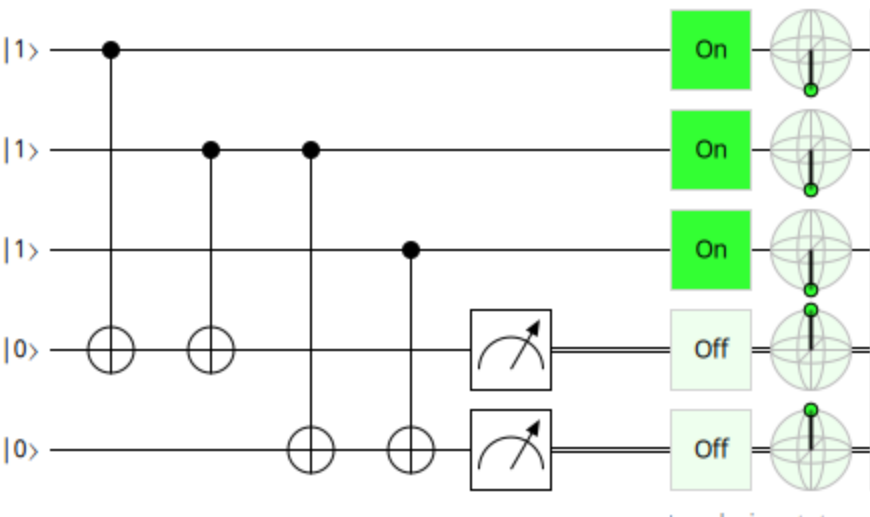
\includegraphics[scale=0.2]{./img/bitflipSyndromeExtraction3Rep.png}\\
	\caption{Bitflip Syndrome extractor\\
        +1 measurement result on first Ancilla indicates a bitflip error
        on qubits 1 or 2, +1 result on second ancilla indicates 
        bitflip on third or fourth qubit}
	\label{fig: syndrome extractor}
	\end{center}
\end{figure}
\\
This way of encoding information however leaves two notable
issues.

For one, it only detects bitflip, or pauli-X errors occuring on
the stored quantum information. While using Hadamard gate one
could trivially adapt this code to instead detect pauli-Z errors,
it is not possible to use linear codes like the repetition code
to $\em{simultaneously}$ detect pauli-X and pauli-Z errors occuring.

Secondly, it also assumes a noise model of a ``Noisy Channel'',
which is not compatible with the actually encountered errors in
real physical quantum computers.

\subsubsection{2D Codes}
Again, the previous research in computer science is of immense
value to us here, providing a toolset for generating valid codes
from existing encoding schemes. 
According to SUCHANDSUCH a hypergraph product code of two 
existing codes will always remain a valid detection code.
We can therefore form hypergraph product code of two repetition
codes for X error detection and Z error detection respectively,
obtaining the so-called ``Surface-Code'' which can detect
$both$ X and Z errors, and therefore any pauli error happening.

PUT IN A NICE DRAWING OF THE SURFACE CODE.
